% This file was created with tikzplotlib v0.10.1.
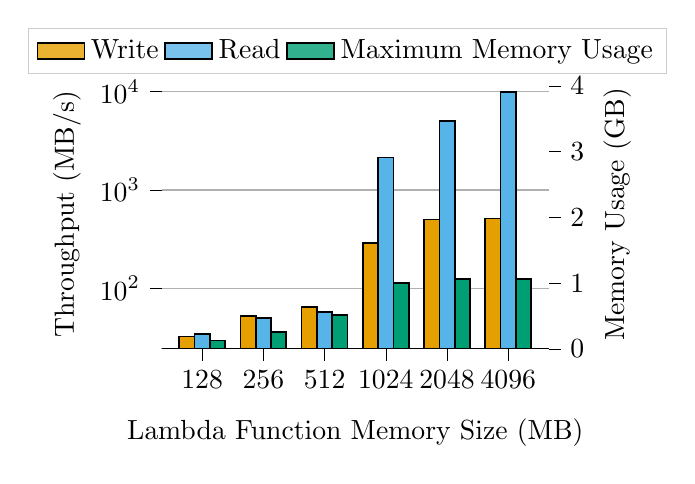
\begin{tikzpicture}

  \definecolor{cornflowerblue86180233}{RGB}{86,180,233}
  \definecolor{darkcyan0158115}{RGB}{0,158,115}
  \definecolor{darkgray176}{RGB}{176,176,176}
  \definecolor{lightgray204}{RGB}{204,204,204}
  \definecolor{orange2301590}{RGB}{230,159,0}

  \begin{axis}[
  height=5cm,
  axis line style={draw=none},
  axis x line*=bottom,
  log basis y={10},
  tick align=outside,
  legend columns=3,
  legend style={
        fill opacity=0.8,
        draw opacity=1,
        text opacity=1,
        at={(0.48,1.02)},
        anchor=south,
        draw=lightgray204
      },
  xlabel style={yshift=-0.1475cm},
  %ylabel style={yshift=-0.3cm},
  tick pos=left,
  width=6.5cm,
  x grid style={darkgray176},
  xlabel={Lambda Function Memory Size (MB)},
  xmin=-0.6625, xmax=5.6625,
  xtick style={color=black},
  xtick={0,1,2,3,4,5},
  xticklabels={128,256,512,1024,2048,4096},
  y grid style={darkgray176},
  ylabel={Throughput (MB/s)},
  ymajorgrids,
  ymin=24.339238705896, ymax=13211.1940295507,
  ymode=log,
  ytick style={color=black},
  ytick={1,10,100,1000,10000,100000,1000000},
  yticklabels={
    \(\displaystyle {10^{0}}\),
    \(\displaystyle {10^{1}}\),
    \(\displaystyle {10^{2}}\),
    \(\displaystyle {10^{3}}\),
    \(\displaystyle {10^{4}}\),
    \(\displaystyle {10^{5}}\),
    \(\displaystyle {10^{6}}\)
  }
  ]
  \draw[draw=black,fill=orange2301590,semithick] (axis cs:-0.375,0) rectangle (axis cs:-0.125,32.4047432378991);
  \addlegendimage{area legend,draw=black,fill=orange2301590,semithick}
  \addlegendentry{Write}

  \draw[draw=black,fill=orange2301590,semithick] (axis cs:0.625,0) rectangle (axis cs:0.875,52.6827717140424);
  \draw[draw=black,fill=orange2301590,semithick] (axis cs:1.625,0) rectangle (axis cs:1.875,65.0081256487657);
  \draw[draw=black,fill=orange2301590,semithick] (axis cs:2.625,0) rectangle (axis cs:2.875,291.438972332541);
  \draw[draw=black,fill=orange2301590,semithick] (axis cs:3.625,0) rectangle (axis cs:3.875,501.322593770957);
  \draw[draw=black,fill=orange2301590,semithick] (axis cs:4.625,0) rectangle (axis cs:4.875,512.048782375448);
  \draw[draw=black,fill=cornflowerblue86180233,semithick] (axis cs:-0.125,0) rectangle (axis cs:0.125,34.2677382161858);
  \addlegendimage{area legend,draw=black,fill=cornflowerblue86180233,semithick}
  \addlegendentry{Read}
  \addlegendimage{area legend,draw=black,fill=darkcyan0158115,semithick}
  \addlegendentry{Maximum Memory Usage}
  \draw[draw=black,fill=cornflowerblue86180233,semithick] (axis cs:0.875,0) rectangle (axis cs:1.125,50.2351648519137);
  \draw[draw=black,fill=cornflowerblue86180233,semithick] (axis cs:1.875,0) rectangle (axis cs:2.125,57.8396886022326);
  \draw[draw=black,fill=cornflowerblue86180233,semithick] (axis cs:2.875,0) rectangle (axis cs:3.125,2131.79134647518);
  \draw[draw=black,fill=cornflowerblue86180233,semithick] (axis cs:3.875,0) rectangle (axis cs:4.125,4998.03436679668);
  \draw[draw=black,fill=cornflowerblue86180233,semithick] (axis cs:4.875,0) rectangle (axis cs:5.125,9922.94253697624);
  \end{axis}

  \begin{axis}[
  axis y line=right,
  axis line style={draw=none},
  axis x line*=bottom,
  height=5cm,
  tick align=outside,
  width=6.5cm,
  x grid style={darkgray176},
  xmin=-0.6625, xmax=5.6625,
  xtick pos=left,
  xtick style={color=black},
  xtick={0,1,2,3,4,5},
  xticklabels={},
  y grid style={darkgray176},
  ylabel={Memory Usage (GB)},
  ymin=0, ymax=4.096,
  ytick pos=right,
  ytick style={color=black},
  %ylabel style={yshift=+0.4cm},
  yticklabel style={anchor=west},
  y axis line style={-}
  ]
  \draw[draw=black,fill=darkcyan0158115,semithick] (axis cs:0.125,0) rectangle (axis cs:0.375,0.128);

  \draw[draw=black,fill=darkcyan0158115,semithick] (axis cs:1.125,0) rectangle (axis cs:1.375,0.256);
  \draw[draw=black,fill=darkcyan0158115,semithick] (axis cs:2.125,0) rectangle (axis cs:2.375,0.512);
  \draw[draw=black,fill=darkcyan0158115,semithick] (axis cs:3.125,0) rectangle (axis cs:3.375,1.002);
  \draw[draw=black,fill=darkcyan0158115,semithick] (axis cs:4.125,0) rectangle (axis cs:4.375,1.062);
  \draw[draw=black,fill=darkcyan0158115,semithick] (axis cs:5.125,0) rectangle (axis cs:5.375,1.063);

  \draw[draw=black] (axis cs:-1.0,0.001) -- (axis cs:16.0,0.001);
  \end{axis}

  \end{tikzpicture}
